
Полученные данные (рис. \ref{fig:motload}a) аппроксимируется зависимостью, вида
\begin{equation}
	F(t) = \sub{N}{max} \left(1- e^{-\sub{t}{load}/\tau}\right),
\end{equation}
где $\tau$ -- характерное время загрузки, $\sub{N}{max}$ -- предельное число атомов.  Построив зависимость $\sub{N}{max} (\delta \nu)$ (рис. \ref{fig:motload}b) можем определить оптимальное значене отстройки $\delta \nu$. 

\begin{figure}[h]
    \centering
    \subfigure[]{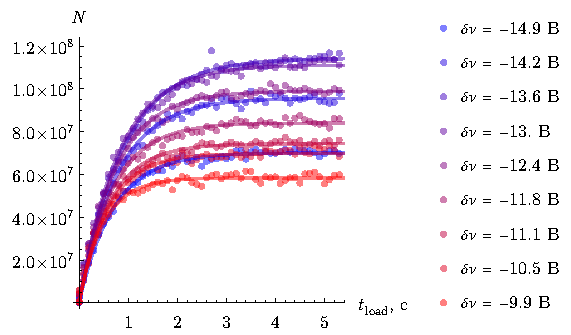
\includegraphics{figs/motload.pdf}}
    \hspace{15 mm} 
    \subfigure[]{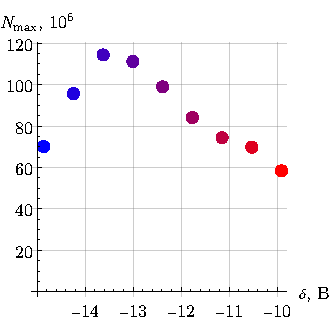
\includegraphics{figs/motload2.pdf}}
    \caption{a) Динамика загрузки МОЛ для различных значений отстройки b)  Зависимость максимального числа атомов в МОЛ от величины отстройки $\delta \nu$}
    \label{fig:motload}
\end{figure}

% для существующей МОЛ поварьировали отстройки, нашли оптимум


